\documentclass[aps,prb,reprint,nofootinbib,a4paper]{revtex4-2}

\usepackage{amsmath,amssymb}
\usepackage{booktabs}
\usepackage{tikz}
\usepackage{xcolor}
\usepackage[protrusion=true,expansion=false]{microtype}
\usepackage{enumitem}
\usepackage[colorlinks=true,linkcolor=blue!55!black,urlcolor=blue!55!black]{hyperref}
\usetikzlibrary{positioning,fit,calc}

\setlength{\emergencystretch}{3em}
\hyphenpenalty=1200
\setlist[itemize]{leftmargin=1.1em,itemsep=1pt,topsep=2pt,parsep=0pt}
\setlist[enumerate]{leftmargin=1.4em,itemsep=1pt,topsep=2pt,parsep=0pt}

\definecolor{cstruct}{RGB}{20,90,170}
\definecolor{clex}{RGB}{190,80,20}
\definecolor{cbad}{RGB}{170,30,40}
\definecolor{cgood}{RGB}{25,120,60}
\definecolor{cgrey}{RGB}{120,120,120}

\newcommand{\code}[1]{\texttt{\small #1}}

\begin{document}

\title{Lumos: LLM Steering for text simplification}
\author{}
\noaffiliation
\date{30 July 2026}

\begin{abstract}
Which levers make a language model simplify text without changing what it
says, and which survive a change of scale? We measure four on
\code{gemma-4-12B-it} and \code{Llama-3.2-3B-Instruct}: a plain simplify
instruction, five worked examples in the prompt, a rank-16 LoRA adapter, and
activation steering, in which a vector estimated once from the model's own
activations is added to its residual stream during generation, scaled by a
strength $\alpha$; plus best-of-$n$ selection over steered candidates.

Two work at both scales. The adapter is the strongest condition on both
models, $+8.47$ and $+6.19$ SARI with intervals clear of zero, and the worked
examples are a real gain on both, $+3.85$ and $+3.44$. Steering is a tie
against no intervention on sentences at both scales, $+0.43$ and $+2.02$ with
intervals across zero. On scientific abstracts it is the strongest condition
on Gemma, $-5.36$ reading grades at a faithfulness change of $-0.05$ whose
interval crosses zero, and real on Llama, $-5.14$ grades at $-0.18$; on 32
longer passages the same condition costs faithfulness, $-0.14$, so the
abstract null reflects $n=10$. Spreading the steering budget over three
adjacent layers gives the only significant steering gain on sentences, $+2.70$
against a tie for one layer, measured on Gemma only.

Two levers change sign with scale. Prompting the 3B model to simplify deletes
facts: $-5.04$ SARI at faithfulness $0.464$, worse than leaving the text
alone. The same instruction on the 12B model gains $+2.91$ at no measurable
faithfulness cost, and a control attributes at most a quarter of the gap to
its wording. Best-of-$n$ is a tie on Llama, $+0.78$, and significant on Gemma,
$+1.82$. The failure that made steering look necessary is a property of the
smaller model.
\end{abstract}

\maketitle

\section{Introduction}

A student who cannot read a textbook paragraph needs it rewritten, and the
rewrite must say the same thing. A language model asked to simplify can drop a
qualifier or invent an example. Whether it does depends on the model's size,
and that dependence is the subject of this paper.

A language model is a program that, given text, predicts what comes next one
\emph{token} at a time, a token being a word or a piece of one; it writes by
repeating that prediction. An \emph{instruction-tuned} model has been further
trained to answer requests, so it can be handed a passage and a sentence such
as \emph{Make this easier to read}. Sentence and passage together are the
\emph{prompt}.

The prompt is the cheapest lever, and it is discrete: the instruction either
takes effect or does not, and its degree is not addressable. Activation
steering supplies a continuous strength. Inside the model each token is a
vector in a space of a few thousand dimensions, and each layer adds a
correction to that vector rather than replacing it; the running sum is the
\emph{residual stream} (\S\ref{sec:background}). If ``simpler'' corresponds to
a direction $v$ in that space, we can estimate $v$ once, offline, from the
model's own \emph{activations}, the stream vectors it produces on chosen
inputs, and add $\alpha v$ to the stream while the model writes. Nothing is
retrained. Control tokens~\cite{access,muss} also make simplification
controllable, but need a training run.

\paragraph{Models and scope.} \code{gemma-4-12B-it} (12 billion parameters, 48
layers) carries the results. Every headline measurement is repeated on
\code{Llama-3.2-3B-Instruct} (3 billion, 28 layers, a different family) to
learn which effects survive a change of model. Steering is compared with the
plain instruction, five worked examples in the prompt, a LoRA adapter and
best-of-$n$ selection. We report only what worked on both models and what
worked on one and failed on the other; the repository's \code{report.md} and
\code{fail.md} record every other condition measured.

\paragraph{Contributions.}
\begin{enumerate}
\item A steering vector for syntactic simplification with depth-normalised
strength, located on both models: layer 15 of 28 on Llama and 31 of 48 on
Gemma, where layers 12--26 collapse at strengths that are safe on Llama
(\S\ref{sec:depth}).
\item What works at both scales: the adapter and the worked examples on
sentences, and steering on long inputs, where on sentences it is a tie at both
scales (\S\ref{sec:eval}, \S\ref{sec:long}).
\item Two levers that change sign with scale, prompting and best-of-$n$, with a
control attributing prompting's failure to the model rather than to the
instruction (\S\ref{sec:eval}, \S\ref{sec:bound}).
\item A depth schedule that works at one scale and is untested at the other
(\S\ref{sec:sched}).
\item An evaluation protocol whose obvious alternatives fail: simplicity
scores that broken text maximises, a grade formula invalid at sentence length,
and one-directional faithfulness that can be gamed (\S\ref{sec:metrics}).
\end{enumerate}

\section{Background}
\label{sec:background}

Both models are \emph{decoder-only transformers}: a stack of $L$ layers of
identical shape that reads a sequence of tokens and predicts the next one. Each
token position holds one vector of width $d$ ($3840$ on Gemma, $3072$ on
Llama). Layer $l$ reads that vector, computes two updates and \emph{adds} them
back:
\begin{equation}
h_{l+1} = h_l + \mathrm{Attn}_l(h_l) + \mathrm{MLP}_l(h_l).
\end{equation}
Attention lets a position draw on the vectors at earlier positions; the MLP, a
small feed-forward network, transforms each position on its own. The stream is
therefore a running sum, and a vector added at layer $l$ persists into every
later layer unless something cancels it. After the last layer the
\emph{unembedding} maps the final vector to a score per vocabulary token; under
\emph{greedy decoding}, used throughout, the model emits the highest-scoring
token, so a prompt always yields the same text.

If a property of the output is represented approximately linearly, some
direction $v$ moves it, and activation steering adds that direction during
generation:
\begin{equation}
h_l \leftarrow h_l + \alpha v .
\label{eq:steer}
\end{equation}
Contrastive activation addition~\cite{caa} estimates $v$ as the mean difference
between the stream vectors of paired inputs that differ in the property;
instruction-following variants pair inputs that differ by the presence of an
instruction~\cite{stolfo2025}. Earlier work reads and writes the same
representations for behavioural control~\cite{repe,actadd,iti}, and
EasySteer~\cite{easysteer} catalogues the estimators.

\section{Method}

\subsection{The steering vector}
\label{sec:est}

For each of $N$ texts $x_i$ we run two forward passes whose prompts differ in
exactly one instruction, $q$ against a placebo $\bar q$ of the same length and
tone that asks for the opposite along the same axis, and average the difference
of the stream vectors at the final prompt position:
\begin{equation}
v_l = \frac{1}{N}\sum_{i=1}^{N}
      \bigl[h_l(x_i \oplus q) - h_l(x_i \oplus \bar q)\bigr].
\label{eq:idiff}
\end{equation}
Both prompts end in the same generation-prompt token, the marker that tells the
model to begin its answer, so that position holds the state the model answers
from and the difference isolates the instruction's effect on it. The placebo,
rather than no instruction, is meant to cancel the part of the difference that
reflects only a shorter prompt. Table~\ref{tab:prompts} gives the prompts
verbatim. The task sentence is always present, because an instruction-tuned
model handed a bare paragraph comments on it rather than rewriting it.

At generation the vector is added on generated positions only, at one layer,
and the stream is rescaled to its original norm afterwards. Adding it at the
final prompt position alone would change the state the model starts from and
then let it run; a continuous strength needs the pressure held on for the whole
output.

\begin{table}[t]
\centering
\small
\caption{The prompts. The task sentence is always present and is never
differenced; on Gemma it carries the suffix given in \S\ref{sec:setup}. The
placebo matches the instruction in length and tone and asks for the opposite
along the same axis.}
\begin{tabular}{@{}p{0.95\columnwidth}@{}}
\toprule
\textbf{Task, always present} \\
\emph{Rewrite the following text.} \\
\midrule
\textbf{Instruction $q$} \\
\emph{Use short, simple sentences with one idea each. Keep every fact exactly as
it is.} \\
\textbf{Placebo $\bar q$} \\
\emph{Keep the original sentence structure and sentence length exactly as they
are.} \\
\midrule
\textbf{Prompted condition} \\
\emph{Make it easy to read for a young student. Do not change the meaning and do
not leave out any information.} \\
\bottomrule
\end{tabular}
\label{tab:prompts}
\end{table}

\subsection{Depth-normalised strength}
\label{sec:scale}

The norm of the residual stream grows with depth: on Llama the measured mean
rises from $1.60$ at layer 0 to $52.04$ at layer 27 (Fig.~\ref{fig:refnorm}).
A raw $\alpha$ is therefore a small nudge early and an overwrite late. Each
stored bank of vectors records the mean norm per layer, and we inject
\begin{equation}
\alpha \cdot \frac{v_l}{\lVert v_l\rVert} \cdot \bar n_l,
\qquad \bar n_l = \mathbb{E}\bigl[\lVert h_l \rVert\bigr].
\label{eq:scale}
\end{equation}
so that $\alpha$ means \emph{this fraction of a typical stream magnitude at
this layer}. Every $\alpha$ in this paper is that quantity. It is comparable
across the depth of one model, not between models (\S\ref{sec:depth}).

\begin{figure}[t]
\centering
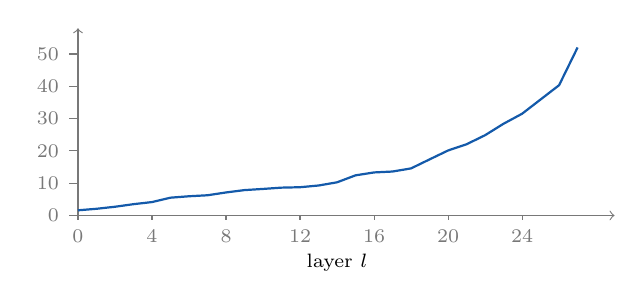
\begin{tikzpicture}[x=0.235cm,y=0.041cm,font=\scriptsize]
  \draw[->,cgrey] (0,0) -- (29,0);
  \draw[->,cgrey] (0,0) -- (0,58);
  \foreach \x in {0,4,8,12,16,20,24} \draw[cgrey] (\x,0) -- (\x,-1.5) node[below]{\x};
  \foreach \y in {0,10,20,30,40,50} \draw[cgrey] (0,\y) -- (-0.5,\y) node[left]{\y};
  \node[below=3.6mm of {(14,0)}] {layer $l$};
  \draw[thick,cstruct] plot coordinates {
    (0,1.60)(1,2.07)(2,2.70)(3,3.50)(4,4.15)(5,5.51)(6,5.95)(7,6.26)(8,7.13)
    (9,7.86)(10,8.22)(11,8.62)(12,8.75)(13,9.28)(14,10.27)(15,12.43)(16,13.33)
    (17,13.61)(18,14.58)(19,17.37)(20,20.13)(21,22.06)(22,24.86)(23,28.42)
    (24,31.51)(25,35.93)(26,40.35)(27,52.04)};
\end{tikzpicture}
\caption{Mean residual norm $\bar n_l$ by layer on Llama, over the 256
estimation texts: $33\times$ growth, which Equation~\ref{eq:scale} divides out.}
\label{fig:refnorm}
\end{figure}

\section{Evaluation protocol}
\label{sec:metrics}

Simplicity is read from words per sentence and from the \emph{Flesch-Kincaid
grade level} (FKGL), which combines words per sentence with syllables per word
into a US school grade. Meaning is scored by \emph{natural language inference}
(NLI), a classifier that, given two sentences, estimates the probability that
the first implies the second; we call that score \emph{faithfulness} and run it
in both directions (\S\ref{sec:nli}). Quality on sentences is SARI~\cite{sari},
the standard simplification score: it compares the output's $n$-grams, runs of
$n$ consecutive words for $n$ from 1 to 4, against the source and against ten
human rewrites, and credits the words the output adds, keeps and deletes in
agreement with the humans. \emph{Degenerate output} is text that has stopped
being text, a phrase repeated to the token limit, a fragment, an empty string,
and is detected by the rules of Table~\ref{tab:degen}. Conditional perplexity,
the model's own measure of how predictable its output is, is reported as a
ratio to the unsteered output's value and never thresholded: it is computed
under the base model, so a condition that legitimately shifts the output
distribution is penalised for succeeding. On Gemma the prompted condition posts
a ratio of $11.11$ with faithfulness $0.95$ and no degenerate output.

\subsection{Simplicity is scored on survivors only}
\label{sec:gate}

Every simplicity metric is maximised by broken text: a Llama rewrite steered
at $\alpha=1.5$ collapsed into a repeating list and scored FKGL $1.72$, the
best grade in its strength ladder. Simplicity is therefore credited only on
outputs that pass the degeneracy rules, and the survivor count is reported with
every cell.

The rules are deliberately narrow, because legitimate simplification also
lowers diversity: the valid group \emph{The cell makes energy. The cell uses
energy. The cell needs energy.} has a type-token ratio, distinct words over
total words, of $0.5$, and 45\% of its adjacent word pairs repeat. The
discriminating signal is a phrase repeated back to back, counted per sentence,
with function-word loops such as \emph{on and on and on} exempt. Perplexity
cannot substitute: a loop is cheaper under the model than prose, $18.8$ for a
broken fragment against $37.0$ for the group above~\cite{holtzman2020}. The
rule set gives zero false positives and zero false negatives on 13 hand-built
cases and 24 real paragraphs.

\begin{table}[t]
\centering
\small
\caption{Degeneracy rules. Diversity thresholds sit low because legitimate
simplification reduces diversity; the discriminating signal is immediate
repetition.}
\begin{tabular}{@{}llr@{}}
\toprule
Rule & Fires when & Value \\
\midrule
\code{too\_short}        & word count below       & 3 \\
\code{punct\_heavy}      & non-alphanumeric above & 0.30 \\
\code{loop\_$n$gram}     & immediate repeat, per sentence & see text \\
\code{low\_diversity}    & distinct-1 below       & 0.35 \\
\code{token\_dominance}  & top token share above  & 0.45 \\
\code{repeated\_bigrams} & repeated bigram share above & 0.60 \\
\code{no\_terminator}    & no \code{.!?} and words above & 30 \\
\bottomrule
\end{tabular}
\label{tab:degen}
\end{table}

\subsection{FKGL is invalid on single sentences}
\label{sec:fkgl}

FKGL is $0.39\,(W/S) + 11.8\,(Y/W) - 15.59$ for $W$ words, $S$ sentences and
$Y$ syllables. On a single sentence $S=1$, so the first term is the sentence's
own word count and the formula rewards splitting and padding. The effect
inverts conclusions: a faithful 17-word paraphrase at faithfulness $0.990$
scored grade $14.3$, and a 60-word rewrite that invented three entities at
$0.090$ scored $7.0$ (Case 1 of Table~\ref{tab:qual}). Tanprasert and
Kauchak~\cite{tanprasert2021} made the same argument, and Flesch-based scores
have the lowest correlation with human judgement in the metric
survey~\cite{alvamanchego2021}. Sentence-level claims here rest on SARI and the
faithfulness threshold; FKGL is interpreted only for passages.

\subsection{Faithfulness needs both directions}
\label{sec:nli}

We score faithfulness with an NLI classifier trained on MNLI, the standard
corpus, run with the source as premise and the output as hypothesis and then
the reverse. If only the source must imply the output, deleting content scores
well, because a shorter claim is easier to imply; if only the output must imply
the source, inventing content scores well. Requiring both bounds omission and
invention at once, and an output passes the threshold when both directions
score at least $0.50$. Scoring is per sentence, so one dropped fact shows up in
the minimum rather than averaging away. NLI penalises heavy paraphrase, so a
low score means lost information or aggressive rewording without saying which;
\S\ref{sec:bound} inspects outputs directly for that reason.

\section{Experimental setup}
\label{sec:setup}

\paragraph{Models.} \code{gemma-4-12B-it}: 48 layers, stream width 3840.
\code{Llama-3.2-3B-Instruct}: 28 layers, width 3072. Both run in half
precision under greedy decoding, seed 0, batch size 8, with
\code{FacebookAI/roberta-large-mnli} for faithfulness. Given the bare task
sentence, Gemma answers with a menu of options rather than a rewrite, so its
task sentence carries the suffix \emph{Reply with the rewritten text only,
nothing else.}; \S\ref{sec:bound} tests whether that suffix explains anything.

\paragraph{Correctness checks.} The code that reads the stream and the code
that writes it were verified against independently built second measurements
before use: $\alpha=0$ reproduces the unsteered output token for token, norm
preservation holds to within half-precision rounding, each position mode fires
where its name says, and the recorded vector matches a separate capture of the
same quantity to cosine $1.000000$. A recorder can pass every internal check
and still read the wrong memory; only an independent capture shows that.

\paragraph{Evaluation sets.} ASSET~\cite{asset} supplies 359 test and 2000
validation sentences with 10 human rewrites each; we evaluate on the first 32
test sentences. Ten arXiv abstracts, one per field, and 32 SQuAD passages of
comparable length carry no rewrites, so SARI is unavailable there and
faithfulness carries the measurement; an abstract is several dependent clauses
of domain vocabulary, where dropping one is easy and invisible to a grade
formula. The vector is estimated from 256 texts drawn from a 665-item filtered
pool of ASSET validation sources, with disjointness from the test set
recomputed on every call; sweep texts are a further 12 or 48 after that slice.
Passages come from an 11\,854-paragraph pool, of which 2 were dropped for
containing an ASSET sentence verbatim.

\paragraph{Conditions.} Every condition carries the task sentence and is
compared against \emph{no intervention}, the task sentence alone, which is the
baseline. Figure~\ref{fig:sites} shows where each enters the model.
\begin{itemize}
\item \emph{prompted}: the simplify instruction of Table~\ref{tab:prompts};
\item \emph{few-shot}: five worked source-to-rewrite examples from ASSET
validation, placed in the prompt as prior turns of the conversation, each using
its source's median-length human rewrite because the shortest usually dropped
a clause;
\item \emph{LoRA}: a low-rank adapter, a small set of trained weight
corrections added to the frozen model, of rank 16, trained on 3800 ASSET
validation pairs with 200 held out;
\item \emph{steered}: the vector of \S\ref{sec:est} at the model's site and
strength, no simplify instruction;
\item \emph{best-of-$n$}: seven candidates per item, the baseline and prompted
rewrites and steered rewrites at several strengths, screened by the degeneracy
rules, the faithfulness threshold and a perplexity ceiling, shipping the
lowest-FKGL survivor; no human rewrite is consulted, so it is deployable.
\end{itemize}
Every metric is computed with the adapter and the vector switched off, and the
baseline text is cached once per model, so every condition is scored against
byte-identical strings.

\begin{figure}[t]
\centering
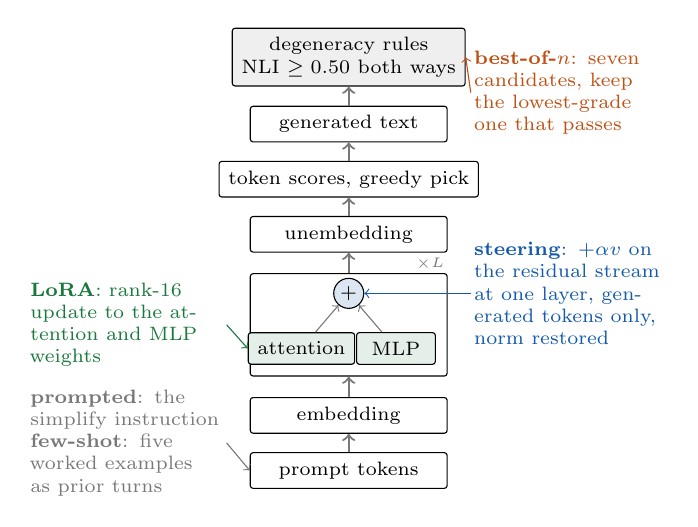
\begin{tikzpicture}[font=\scriptsize,
  blk/.style={draw,rounded corners=1pt,minimum width=2.5cm,minimum height=4.4mm,align=center},
  sub/.style={draw,rounded corners=1pt,minimum width=1.0cm,minimum height=3.8mm,align=center,fill=cgood!12},
  note/.style={align=left,text width=2.45cm,inner sep=1pt,font=\scriptsize}]
  \node[blk] (in) at (0,0) {prompt tokens};
  \node[blk] (emb) at (0,0.7) {embedding};
  \node[draw,rounded corners=1pt,minimum width=2.5cm,minimum height=1.3cm] (layer) at (0,1.85) {};
  \node[sub] (att) at (-0.6,1.55) {attention};
  \node[sub] (mlp) at (0.6,1.55) {MLP};
  \node[draw,circle,inner sep=1pt,fill=cstruct!15] (sum) at (0,2.25) {$+$};
  \node[font=\tiny,cgrey,anchor=south east,inner sep=1pt] at (layer.north east) {$\times L$};
  \node[blk] (unemb) at (0,3.0) {unembedding};
  \node[blk] (dec) at (0,3.7) {token scores, greedy pick};
  \node[blk] (out) at (0,4.4) {generated text};
  \node[blk,fill=cgrey!12,minimum height=7mm] (chk) at (0,5.25) {degeneracy rules\\NLI $\ge 0.50$ both ways};
  \draw[->,thick,cgrey] (in) -- (emb);
  \draw[->,thick,cgrey] (emb) -- (layer);
  \draw[->,thick,cgrey] (layer) -- (unemb);
  \draw[->,thick,cgrey] (unemb) -- (dec);
  \draw[->,thick,cgrey] (dec) -- (out);
  \draw[->,thick,cgrey] (out) -- (chk);
  \draw[->,cgrey] (att) -- (sum);
  \draw[->,cgrey] (mlp) -- (sum);
  \node[note,anchor=east,cgrey] (n1) at (-1.55,0.35) {\textbf{prompted}: the simplify instruction\\\textbf{few-shot}: five worked examples as prior turns};
  \draw[->,cgrey] (n1.east) -- (in.west);
  \node[note,anchor=east,cgood] (n2) at (-1.55,1.85) {\textbf{LoRA}: rank-16 update to the attention and MLP weights};
  \draw[->,cgood] (n2.east) -- (att.west);
  \node[note,anchor=west,cstruct] (n3) at (1.55,2.25) {\textbf{steering}: $+\alpha v$ on the residual stream at one layer, generated tokens only, norm restored};
  \draw[->,cstruct] (n3.west) -- (sum.east);
  \node[note,anchor=west,clex] (n4) at (1.55,4.8) {\textbf{best-of-$n$}: seven candidates, keep the lowest-grade one that passes};
  \draw[->,clex] (n4.west) -- (chk.east);
\end{tikzpicture}
\caption{Where each condition enters. Prompting and few-shot change the input
tokens; the adapter changes weights inside every layer; steering adds a vector
to the residual stream at one layer; best-of-$n$ selects after generation,
using the two checks every output passes through.}
\label{fig:sites}
\end{figure}

\paragraph{Settings.} Estimation uses $N=256$. On Llama a coarse sweep screens
$\alpha \in \{0.5, 1.0\}$ over all 28 layers at 12 texts per cell and a finer
strength grid runs on the top 3 layers; on Gemma the same coarse screen covers
all 48 layers and a second stage runs at lower $\alpha$, because both coarse
strengths break it (\S\ref{sec:depth}). A cell is eligible if no output is
degenerate, the faithfulness threshold passes on at least 75\% of items, and
the sentence-length reduction is at least $0.05$; the last floor is needed
because a selectivity score alone ranks an inert cell first. Sweeps generate
96 tokens and evaluations 320, and every effect is measured against the same
text's own unsteered rewrite. The sites used are layer 15 at $\alpha=0.75$ on
Llama and layer 31 at $\alpha=0.5$ on Gemma. Gemma's $\alpha=1.0$ was rejected
on faithfulness, not fluency: re-screened at 320 tokens it does not degenerate
but scores $0.260$ against $0.858$ at $\alpha=0.5$. The two settings were not
chosen alike, Gemma's by a selector corrected to require a measured
faithfulness score and Llama's by the earlier process, so an unknown part of
the gap between the models' steering results is setting quality rather than
model capability.

\paragraph{Statistics.} Every comparison is paired within item: for each item
we take the difference between a condition's score and the baseline's and ask
whether the mean difference is distinguishable from zero. The 95\% intervals
are \emph{paired bootstrap confidence intervals}, obtained by resampling the
items with replacement many times and taking the middle 95\% of the recomputed
means. An interval containing zero is reported as a tie; $^*$ marks one that
excludes it.

\section{Results}
\label{sec:results}

\subsection{Where the vector acts, at each scale}
\label{sec:depth}

On Llama the vector reduces sentence length only when injected in layers
10--18, and nowhere else at any strength tested; the site used, layer 15, sits
at 54\% of depth. Its sign is correct, at $\alpha=-1.0$ the layer-17 vector
\emph{lengthens} sentences by 60\%, and its response is not monotone: the
layer-17 effect peaks at $+0.339$ at $\alpha=1.0$ and collapses to $+0.027$ at
$1.25$ as degeneration sets in, the coefficient sensitivity Braun et
al.~\cite{braun2025} report as general.

On Gemma the site is layer 31, at 65\% of depth, and the profile is a cliff
rather than a band (Fig.~\ref{fig:depthmap}). Layers 0--11 do nothing, every
cell within $\pm 0.008$ with no degenerate output; layer 12 jumps to an effect
of $0.50$ to $0.73$ with 92\% of outputs degenerate. At $\alpha=0.5$ and
$1.0$, both safe on Llama, layers 12--26 degenerate 33\% to 92\% of outputs,
and two cells lost all twelve of their texts. Depth normalisation
(\S\ref{sec:scale}) therefore does not make a strength portable between
models; Gemma needed its own second sweep stage.

\begin{figure}[t]
\centering
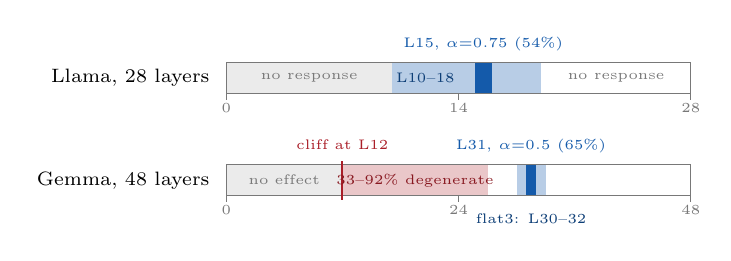
\begin{tikzpicture}[x=5.9cm,y=1cm,font=\scriptsize]
  \fill[cgrey!15] (0,1.3) rectangle (10/28,1.7);
  \fill[cstruct!30] (10/28,1.3) rectangle (19/28,1.7);
  \fill[cstruct] (15/28,1.3) rectangle (16/28,1.7);
  \draw[cgrey] (0,1.3) rectangle (1,1.7);
  \node[anchor=east] at (-0.015,1.5) {Llama, 28 layers};
  \node[font=\tiny,cgrey] at (5/28,1.5) {no response};
  \node[font=\tiny,cstruct!70!black] at (12/28,1.5) {L10--18};
  \node[font=\tiny,cgrey] at (23.5/28,1.5) {no response};
  \node[font=\tiny,cstruct,anchor=south] at (15.5/28,1.72) {L15, $\alpha{=}0.75$ (54\%)};
  \foreach \l in {0,14,28} \draw[cgrey] (\l/28,1.3) -- (\l/28,1.22) node[below,font=\tiny,inner sep=1pt]{\l};
  \fill[cgrey!15] (0,0) rectangle (12/48,0.4);
  \fill[cbad!25] (12/48,0) rectangle (27/48,0.4);
  \fill[cstruct!30] (30/48,0) rectangle (33/48,0.4);
  \fill[cstruct] (31/48,0) rectangle (32/48,0.4);
  \draw[cgrey] (0,0) rectangle (1,0.4);
  \draw[cbad,thick] (12/48,-0.05) -- (12/48,0.45);
  \node[anchor=east] at (-0.015,0.2) {Gemma, 48 layers};
  \node[font=\tiny,cgrey] at (6/48,0.2) {no effect};
  \node[font=\tiny,cbad!80!black] at (19.5/48,0.2) {33--92\% degenerate};
  \node[font=\tiny,cbad,anchor=south] at (12/48,0.47) {cliff at L12};
  \node[font=\tiny,cstruct,anchor=south] at (31.5/48,0.42) {L31, $\alpha{=}0.5$ (65\%)};
  \node[font=\tiny,cstruct!70!black,anchor=north] at (31.5/48,-0.1) {flat3: L30--32};
  \foreach \l in {0,24,48} \draw[cgrey] (\l/48,0) -- (\l/48,-0.08) node[below,font=\tiny,inner sep=1pt]{\l};
\end{tikzpicture}
\caption{Depth map of the syntactic vector, layers scaled to each model's
depth. Llama responds only in layers 10--18; the site used is L15. Gemma's
layers 0--11 do nothing at any strength tested, layer 12 is a cliff, and at the
two strengths that are safe on Llama layers 12--26 degenerate 33--92\% of
outputs; the site used is L31 at $\alpha=0.5$, and the schedule of
\S\ref{sec:sched} spreads that budget over L30--32.}
\label{fig:depthmap}
\end{figure}

\subsection{Sentences at two scales}
\label{sec:eval}

Table~\ref{tab:asset} gives the five conditions on ASSET for both models. The
adapter is the strongest condition on both and the worked examples are a real
gain on both. Steering is a tie against no intervention on both, and on Gemma
its faithfulness cost of $-0.01$, though tiny, is resolved; what it does on
Llama is cut sentence length 18\% and grade 19\% at no measurable SARI or
faithfulness cost, which meets the requirement of simplifying without changing
meaning and not the stronger one of improving on the source.

Two conditions change sign. Prompting is significantly worse than doing
nothing on Llama and costs $0.41$ of faithfulness, while on Gemma it gains
quality at a faithfulness change indistinguishable from zero. Best-of-$n$ is a
tie on Llama and significant on Gemma. Its selector never sees a human rewrite,
and it rejects Llama's prompted candidate on the faithfulness floor 22 times in
32 and Gemma's 0 times in 28: the same reference-free check detects prompting's
failure on the model where it exists and declines to flag it on the model where
it does not.

On Llama, steering beats prompting head to head: SARI $+5.47$ with interval
$[+2.58, +8.48]$, 23 items to 9, and faithfulness $+0.33$ with interval
$[+0.20, +0.46]$, 27 to 5. That comparison, not any gain over doing nothing,
is what made steering look necessary at 3B, and it has no counterpart on
Gemma, where prompting's gain is resolved and steering's is not.

\begin{table*}[t]
\centering
\small
\caption{ASSET test, $n=32$ per model, paired per-item differences against no
intervention with 95\% bootstrap intervals; $^*$ marks an interval excluding
zero. No condition here produced degenerate output on either model
(best-of-$n$'s share on Gemma was not recorded). Steering at L15,
$\alpha=0.75$ on Llama and L31, $\alpha=0.5$ on Gemma.}
\begin{tabular}{@{}lrrrr@{}}
\toprule
& \multicolumn{2}{c}{Llama-3.2-3B} & \multicolumn{2}{c}{gemma-4-12B} \\
Condition & $\Delta$SARI & $\Delta$NLI & $\Delta$SARI & $\Delta$NLI \\
\midrule
LoRA        & $+8.47^{*}$ $[6.12,\,10.97]$  & $-0.00$ $[-0.16,\,0.14]$      & $+6.19^{*}$ $[2.81,\,9.32]$ & $-0.07$ $[-0.19,\,0.04]$ \\
few-shot    & $+3.85^{*}$ $[1.57,\,6.19]$   & $+0.06$ $[-0.04,\,0.17]$      & $+3.44^{*}$ $[1.61,\,5.35]$ & $+0.03$ $[-0.00,\,0.09]$ \\
steered     & $+0.43$ $[-1.71,\,2.59]$      & $-0.08$ $[-0.21,\,0.05]$      & $+2.02$ $[-0.32,\,4.32]$    & $-0.01^{*}$ $[-0.03,\,-0.00]$ \\
\midrule
prompted    & $-5.04^{*}$ $[-8.15,\,-2.05]$ & $-0.41^{*}$ $[-0.53,\,-0.29]$ & $+2.91^{*}$ $[0.81,\,4.96]$ & $-0.01$ $[-0.07,\,0.06]$ \\
best-of-$n$ & $+0.78$ $[-0.85,\,2.43]$      & $+0.05$ $[-0.00,\,0.12]$      & $+1.82^{*}$ $[0.49,\,3.37]$ & $-0.01^{*}$ $[-0.04,\,-0.00]$ \\
\bottomrule
\end{tabular}
\label{tab:asset}
\end{table*}

\subsection{Prompting: the lever that changes sign}
\label{sec:bound}

On Llama the plain instruction takes the mean grade from $12.49$ to $6.47$ and
faithfulness from $0.875$ to $0.464$. Table~\ref{tab:qual} shows how: it
reaches the low grade by replacing content, substituting an analogy for a
statistic and dropping the figure. The low faithfulness scores are lost
information, not stylistic distance, which settles the paraphrase concern of
\S\ref{sec:nli}.

Gemma's task sentence carries a suffix that Llama's does not, so ``Gemma does
not delete content'' and ``Gemma was asked more precisely'' were the same
observation. With Gemma's exact sentence, Llama's prompted condition moves
from $-5.04^{*}$ to $-4.96^{*}$ SARI and from $-0.41^{*}$ to $-0.32^{*}$
faithfulness, against Gemma's $+2.91^{*}$ and $-0.01$: it recovers $0.09$ of
the $0.40$ faithfulness gap, about a quarter, and none of the quality gap. On
the abstracts it recovers nothing, Llama's prompted output scoring
faithfulness $0.06$ under its own sentence and $0.07$ under Gemma's against
$0.53$ for Gemma. The harder the source, the more of the difference is model
capability rather than instruction wording. Prompting a model to simplify does
make it delete content; that is a property of the 3B model, and it does not
survive to 12B.

\begin{table*}[t]
\centering
\small
\caption{Two sources on Llama under prompting and under steering.
Case 1 is the inversion of \S\ref{sec:fkgl}: the faithful output scores
\emph{worse} on grade level than the one that invents three entities, because
it is shorter and denser.}
\begin{tabular}{@{}p{1.9cm}p{6.3cm}p{6.3cm}@{}}
\toprule
& Case 1 & Case 2 \\
\midrule
Source &
Some academic journals do refer to Wikipedia articles, but are not elevating it
to the same level as traditional references. &
The aggregate income distribution is highly concentrated towards the top, with
the top 6.37\% earning roughly one third of all income. \\
\addlinespace
Prompt-only &
\emph{You might have noticed that some big schools and universities use Wikipedia
articles in their research\dots they don't think it's as good as other sources,
like books or articles from experts.} &
\emph{Imagine you have a big jar of cookies, and you want to know how the cookies
are divided among the people\dots some groups have a lot more cookies than
others.} \\
& FKGL 7.0, NLI \textbf{0.090}. Universities, books and experts are invented. &
NLI \textbf{0.025}. The 6.37\% figure is gone. \\
\addlinespace
Steered L15, $\alpha{=}0.75$ &
\emph{Some academic journals mention Wikipedia articles, but they do not consider
them equal to traditional references.} &
\emph{The US income distribution is highly skewed towards the top, with the top
6.37\% of earners holding about one-third of the country's total income.} \\
& FKGL 14.3, NLI \textbf{0.990}. Faithful, and simpler wording. &
no-hallucination \textbf{0.63}. Figure retained. \\
\bottomrule
\end{tabular}
\label{tab:qual}
\end{table*}

\subsection{Long inputs}
\label{sec:long}

Sentences are short enough to survive almost any rewrite; Table~\ref{tab:long}
moves to the abstracts and passages, where faithfulness carries the
measurement. On the abstracts steering is the strongest condition on Gemma,
$5.4$ reading grades at a faithfulness change whose interval crosses zero,
where the instruction cuts more at a resolved cost; on Llama the same
condition cuts $5.14$ grades at a resolved cost of $-0.18$, and one of its ten
outputs is degenerate. But $n=10$ is underpowered for a null: $-0.05$ with
interval $[-0.14, 0.03]$ is consistent with a real loss of up to $0.14$, and
on the 32 passages the same Gemma condition reads exactly $-0.14$ with the
interval clear of zero. Steering on long input works at both scales and costs
meaning at both; the abstract tie is what a sample of ten cannot resolve.

The adapter holds meaning on long input at both scales, $-0.03$ on Llama's
abstracts and $-0.02$ on Gemma's passages with both intervals across zero, and
buys the least readability doing so. Few-shot ties on Gemma's passages
($-0.03$) but not on Llama's abstracts ($-0.20^{*}$). Prompting on Llama's
abstracts scores faithfulness $0.06$: it replaces the abstract rather than
simplifying it.

\begin{table}[t]
\centering
\footnotesize
\setlength{\tabcolsep}{4pt}
\caption{Long inputs, paired against no intervention with 95\% bootstrap
intervals; $^*$ marks an interval excluding zero. No human rewrites exist, so
faithfulness (NLI) carries the measurement. Best-of-$n$ was not run here.}
\begin{tabular}{@{}lrr@{}}
\toprule
& $\Delta$FKGL & $\Delta$NLI \\
\midrule
\multicolumn{3}{@{}l}{\emph{Gemma, abstracts, $n=10$}} \\
steered  & $-5.36^{*}$ $[-6.15,\,-4.60]$   & $-0.05$ $[-0.14,\,0.03]$ \\
prompted & $-8.01^{*}$ $[-9.75,\,-6.28]$   & $-0.37^{*}$ $[-0.50,\,-0.22]$ \\
LoRA     & $-2.62^{*}$ $[-3.45,\,-1.65]$   & $-0.11$ $[-0.25,\,0.01]$ \\
few-shot & $-2.06^{*}$ $[-2.90,\,-1.17]$   & $-0.01$ $[-0.09,\,0.05]$ \\
\midrule
\multicolumn{3}{@{}l}{\emph{Gemma, passages, $n=32$}} \\
steered  & $-6.70^{*}$ $[-7.69,\,-5.77]$   & $-0.14^{*}$ $[-0.20,\,-0.07]$ \\
prompted & $-6.64^{*}$ $[-7.41,\,-5.88]$   & $-0.16^{*}$ $[-0.25,\,-0.08]$ \\
LoRA     & $-3.68^{*}$ $[-4.70,\,-2.59]$   & $-0.02$ $[-0.09,\,0.04]$ \\
few-shot & $-2.72^{*}$ $[-3.27,\,-2.21]$   & $-0.03$ $[-0.08,\,0.01]$ \\
\midrule
\multicolumn{3}{@{}l}{\emph{Llama, abstracts, $n=10$}} \\
steered  & $-5.14^{*}$ $[-6.80,\,-3.50]$   & $-0.18^{*}$ $[-0.27,\,-0.09]$ \\
prompted & $-9.84^{*}$ $[-11.24,\,-8.60]$  & $-0.73^{*}$ $[-0.83,\,-0.59]$ \\
LoRA     & $-1.50^{*}$ $[-2.85,\,-0.14]$   & $-0.03$ $[-0.20,\,0.11]$ \\
few-shot & $-3.18^{*}$ $[-4.39,\,-2.15]$   & $-0.20^{*}$ $[-0.33,\,-0.07]$ \\
\bottomrule
\end{tabular}
\label{tab:long}
\end{table}

\subsection{A depth schedule, at one scale}
\label{sec:sched}

The sweep is a grid over (layer, $\alpha$) whose best cell is one pair, which
is not an argument for injecting at one layer. At a fixed budget, is it better
to concentrate the push or to spread it? On Gemma, $\alpha=0.5$ split as
$0.167$ at each of layers 30, 31 and 32 scores $+2.70$ SARI with the interval
clear of zero, against a tie for the single layer (Table~\ref{tab:sched}): the
only significant steering gain on sentences in this study.

The comparison is ambiguous on its own, because norm restoration after each
injection lets a later layer partly undo an earlier one, so the spread lands a
weaker push than the single layer it is matched to ($-1.78$ grades against
$-2.57$) and might only sit at a gentler point on the same curve. The
ablation walks the single layer down to the spread's realised dose: at
$\alpha=0.35$ the two match on grade, $-0.21$ with interval $[-0.58, +0.19]$,
and the spread still wins on quality by $+2.09$ with interval $[+0.98,
+3.41]$. The effect is the shape, not the strength. It is one run at $n=32$ on
one model, with a non-monotone single-layer dose curve underneath it, and it
has not been run on Llama.

\begin{table}[t]
\centering
\caption{Depth schedules on Gemma, ASSET, $n=32$, paired against no
intervention; $^*$ marks a 95\% interval excluding zero. The last row is a
paired head-to-head between the two conditions above it.}
\setlength{\tabcolsep}{2pt}
\scriptsize
\begin{tabular}{@{}lrr@{}}
\toprule
Condition & $\Delta$FKGL & $\Delta$SARI \\
\midrule
single, L31 $\alpha{=}0.500$        & $-2.57^{*}$ & $+1.84$ $[-0.51,\,+4.15]$ \\
single, L31 $\alpha{=}0.350$        & $-1.57^{*}$ & $+0.61$ \\
flat3, L30--32 $\alpha{=}0.167$ & $-1.78^{*}$ & $+2.70^{*}$ $[+0.42,\,+4.98]$ \\
\midrule
flat3 vs.\ single $0.350$ & $-0.21$ $[-0.58,\,+0.19]$ & $+2.09^{*}$ $[+0.98,\,+3.41]$ \\
\bottomrule
\end{tabular}
\label{tab:sched}
\end{table}

\section{Next steps}
\label{sec:next}

\begin{itemize}
\item \textbf{Replicate the depth schedule} on Llama and at larger $n$; it is
the only positive steering result on sentences and rests on one run.
\item \textbf{Settle the sentence ties.} Interval width falls as $1/\sqrt{n}$,
so the full 359-item ASSET test narrows Llama's $\pm 2.15$ SARI to roughly
$\pm 0.64$; \code{src/evaluate.py --n 359} is the whole change, at roughly
eleven times the runtime per model.
\item \textbf{Replace the faithfulness model.} \code{roberta-large-mnli}
penalises paraphrase, so every faithfulness number here is a lower bound and
the steering-versus-baseline ties sit inside that uncertainty.
AlignScore~\cite{alignscore} and SummaC~\cite{summac} are stronger instruments
and the backend is one function.
\item \textbf{Measure comprehension.} Agrawal and Carpuat~\cite{agrawal2024}
ask comprehension questions of the simplified text and find the best supervised
system leaves 14\% unanswerable; OneStopQA~\cite{onestop}, already loaded,
carries such questions per paragraph. It is the only measurement here that
speaks to the actual goal.
\item \textbf{Explain the adapter on long input.} It holds meaning on long
input at both scales and on Llama moves an abstract far less than a sentence;
an adapter that mostly declines to act looks faithful for the wrong reason, and
the cause is open.
\item \textbf{Test domain transfer.} The vector is estimated and evaluated on
ASSET; Braun et al.~\cite{braun2025} report that steering vectors often fail
to generalise across prompt sets, and textbook prose matches neither corpus.
\item \textbf{Ablate depth normalisation.} It demonstrably does not make
$\alpha$ portable between models; whether it changes the within-model depth
profile is untested.
\end{itemize}

\begin{thebibliography}{99}

\bibitem{repe} A. Zou \textit{et al.},
``Representation Engineering: A Top-Down Approach to AI Transparency,''
arXiv:2310.01405 (2023).

\bibitem{actadd} A. M. Turner \textit{et al.},
``Steering Language Models With Activation Engineering,''
arXiv:2308.10248 (2023).

\bibitem{iti} K. Li \textit{et al.},
``Inference-Time Intervention: Eliciting Truthful Answers from a Language Model,''
NeurIPS (2023), arXiv:2306.03341.

\bibitem{caa} N. Rimsky \textit{et al.},
``Steering Llama 2 via Contrastive Activation Addition,''
ACL (2024), arXiv:2312.06681.

\bibitem{stolfo2025} A. Stolfo \textit{et al.},
``Improving Instruction-Following in Language Models through Activation Steering,''
ICLR (2025), arXiv:2410.12877.

\bibitem{easysteer} \textit{EasySteer: A Unified Framework for High-Performance
and Extensible LLM Steering}, arXiv:2509.25175 (2025).

\bibitem{braun2025} J. Braun \textit{et al.},
``Understanding (Un)Reliability of Steering Vectors in Language Models,''
arXiv:2505.22637 (2025).

\bibitem{holtzman2020} A. Holtzman \textit{et al.},
``The Curious Case of Neural Text Degeneration,''
ICLR (2020), arXiv:1904.09751.

\bibitem{sari} W. Xu \textit{et al.},
``Optimizing Statistical Machine Translation for Text Simplification,''
TACL \textbf{4}, 401 (2016).

\bibitem{asset} F. Alva-Manchego \textit{et al.},
``ASSET: A Dataset for Tuning and Evaluation of Sentence Simplification Models
with Multiple Rewriting Transformations,'' ACL (2020).

\bibitem{onestop} S. Vajjala and I. Lu\v{c}i\'c,
``OneStopEnglish Corpus: A New Corpus for Automatic Readability Assessment and
Text Simplification,'' BEA (2018).

\bibitem{tanprasert2021} T. Tanprasert and D. Kauchak,
``Flesch-Kincaid is Not a Text Simplification Evaluation Metric,''
GEM (2021).

\bibitem{alvamanchego2021} F. Alva-Manchego, C. Scarton, and L. Specia,
``The (Un)Suitability of Automatic Evaluation Metrics for Text Simplification,''
Computational Linguistics \textbf{47}, 861 (2021).

\bibitem{agrawal2024} S. Agrawal and M. Carpuat,
``Do Text Simplification Systems Preserve Meaning? A Human Evaluation via Reading
Comprehension,'' TACL (2024), arXiv:2312.10126.

\bibitem{summac} P. Laban \textit{et al.},
``SummaC: Re-Visiting NLI-based Models for Inconsistency Detection in
Summarization,'' TACL \textbf{10}, 163 (2022).

\bibitem{alignscore} Y. Zha \textit{et al.},
``AlignScore: Evaluating Factual Consistency with a Unified Alignment Function,''
ACL (2023).

\bibitem{access} L. Martin \textit{et al.},
``Controllable Sentence Simplification,'' LREC (2020), arXiv:1910.02677.

\bibitem{muss} L. Martin \textit{et al.},
``MUSS: Multilingual Unsupervised Sentence Simplification by Mining
Paraphrases,'' LREC (2022).

\end{thebibliography}

\end{document}
